\documentclass[12pt,a4paper]{article}

%-----------------------------------------------------------
% Packages
%-----------------------------------------------------------
\usepackage[margin=1in]{geometry}
\usepackage{graphicx}
\usepackage{amsmath}
\usepackage{hyperref}
\usepackage{booktabs}
\usepackage{array}
\usepackage{longtable}
\usepackage{xcolor}
\usepackage{titlesec}
\usepackage{fancyhdr}
\usepackage{enumitem}
\usepackage{tikz}
\usetikzlibrary{shapes.geometric, arrows, positioning, fit, backgrounds}
\usepackage{fontenc}
\usepackage{inputenc}
\usepackage{parskip}
\usepackage{microtype}
\usepackage{float}
\usepackage{tabularx}
\usepackage{multirow}
\usepackage{mdframed}

%-----------------------------------------------------------
% Colors
%-----------------------------------------------------------
\definecolor{primaryblue}{RGB}{30, 58, 138}
\definecolor{accentpurple}{RGB}{109, 40, 217}
\definecolor{lightgray}{RGB}{248, 249, 250}
\definecolor{darkgray}{RGB}{55, 65, 81}
\definecolor{successgreen}{RGB}{5, 150, 105}
\definecolor{warningorange}{RGB}{217, 119, 6}

%-----------------------------------------------------------
% Section Formatting
%-----------------------------------------------------------
\titleformat{\section}
  {\Large\bfseries\color{primaryblue}}
  {\thesection.}{0.5em}{}[\titlerule]

\titleformat{\subsection}
  {\large\bfseries\color{accentpurple}}
  {\thesubsection.}{0.5em}{}

\titleformat{\subsubsection}
  {\normalsize\bfseries\color{darkgray}}
  {\thesubsubsection.}{0.5em}{}

%-----------------------------------------------------------
% Header / Footer
%-----------------------------------------------------------
\pagestyle{fancy}
\fancyhf{}
\rhead{\textcolor{primaryblue}{\textit{Technical System Essay}}}
\lhead{\textcolor{primaryblue}{\textbf{WellnessGPT}}}
\rfoot{\thepage}
\lfoot{\textcolor{darkgray}{\footnotesize HeyDoc AI $\cdot$ HeyDoc Healthtech Pvt. Ltd.}}

%-----------------------------------------------------------
% Hyperref Setup
%-----------------------------------------------------------
\hypersetup{
    colorlinks=true,
    linkcolor=primaryblue,
    urlcolor=accentpurple,
    citecolor=successgreen,
    pdftitle={WellnessGPT - Technical System Essay},
    pdfauthor={Research Analysis},
    pdfsubject={Agentic AI for Healthcare}
}

%-----------------------------------------------------------
% Document
%-----------------------------------------------------------
\begin{document}

%-----------------------------------------------------------
% Title Page
%-----------------------------------------------------------
\begin{titlepage}
    \centering
    \vspace*{2cm}

    {\Huge\bfseries\color{primaryblue} WellnessGPT}\\[0.5cm]
    {\Large\color{accentpurple} Technical System Essay (TSE)}\\[0.3cm]
    {\large\color{darkgray} Agentic AI Operating System for Healthcare}\\[2cm]

    \begin{mdframed}[backgroundcolor=lightgray, linecolor=primaryblue, linewidth=1.5pt, roundcorner=5pt]
        \centering
        \vspace{0.3cm}
        \textit{``Healthcare Needs Reliable AI --- WellnessGPT Makes It Possible''}\\[0.3cm]
        \textbf{Website:} \href{https://wellness-gpt.com}{https://wellness-gpt.com}\\
        \textbf{Parent Company:} HeyDoc AI (HeyDoc Healthtech Pvt. Ltd.)\\
        \textbf{Domain:} Healthcare Artificial Intelligence\\
        \textbf{Category:} Enterprise Agentic AI Platform\\
        \vspace{0.3cm}
    \end{mdframed}

    \vspace{2cm}

    \begin{tabular}{ll}
        \textbf{Document Type:} & Technical System Essay \\
        \textbf{Subject:}       & System Analysis \& Architecture \\
        \textbf{Date:}          & March 2026 \\
        \textbf{Version:}       & 1.0 \\
    \end{tabular}

    \vfill

    {\small\color{darkgray} Research conducted on \texttt{wellness-gpt.com} and \texttt{heydoc.co.in}}
\end{titlepage}

%-----------------------------------------------------------
% Table of Contents
%-----------------------------------------------------------
\tableofcontents
\newpage

%-----------------------------------------------------------
% Abstract
%-----------------------------------------------------------
\begin{abstract}
\noindent
This Technical System Essay (TSE) provides a comprehensive analysis of \textbf{WellnessGPT}, an Agentic Artificial Intelligence Operating System developed by HeyDoc AI (HeyDoc Healthtech Pvt. Ltd.) for the healthcare industry. The document examines the platform's three-pillar architecture — Specialized Healthcare AI Agents, Agentic Orchestration Engine, and HealthMem Temporal Memory — along with its system flow, underlying technology stack, compliance framework, integration capabilities, and competitive positioning. WellnessGPT represents a significant departure from generic large language model (LLM) deployments by offering domain-specific agents with longitudinal patient memory, multi-agent orchestration, and regulatory compliance aligned with HIPAA, FHIR, and India's ABDM ecosystem.
\end{abstract}

\newpage

%-----------------------------------------------------------
% Section 1: Introduction
%-----------------------------------------------------------
\section{Introduction}

\subsection{Background}

The proliferation of Large Language Models (LLMs) such as GPT-4 and Gemini has opened new possibilities for natural language understanding and generation across industries. However, their deployment in \textbf{regulated, high-stakes environments like healthcare} presents serious challenges: these models are stateless (no persistent memory), generalist (not clinically specialized), non-compliant by default (no HIPAA or FHIR alignment), and lack structured workflow orchestration.

\textbf{WellnessGPT} emerges as a purpose-built solution to these challenges. Developed by \textbf{HeyDoc AI}, it is an Agentic AI Operating System that provides the infrastructure needed to deploy reliable, compliant, and memory-enabled AI agents across clinical and administrative healthcare workflows.

\subsection{Platform Identity}

\begin{table}[H]
\centering
\renewcommand{\arraystretch}{1.4}
\begin{tabularx}{\textwidth}{lX}
\toprule
\textbf{Attribute} & \textbf{Detail} \\
\midrule
Full Name            & WellnessGPT \\
Platform Type        & Agentic AI Operating System for Healthcare \\
Website              & \href{https://wellness-gpt.com}{wellness-gpt.com} \\
Parent Company       & HeyDoc AI (HeyDoc Healthtech Pvt. Ltd.) \\
Consumer Product     & HeyDoc App (\href{https://heydoc.co.in}{heydoc.co.in}) \\
Target Market        & B2B: Hospitals, Insurers, Digital Health Firms \\
Geography            & India-first; globally aligned (HIPAA, FHIR) \\
Business Model       & Enterprise SaaS (custom pricing) \\
Core Tagline         & ``Healthcare Needs Reliable AI'' \\
\bottomrule
\end{tabularx}
\caption{Platform Identity Summary}
\end{table}

\subsection{Objectives of This Essay}

This TSE aims to:
\begin{enumerate}[noitemsep]
    \item Describe what WellnessGPT is and what problem it solves
    \item Explain the architecture and its three core pillars in technical depth
    \item Map the complete user and system flow
    \item Document the technology stack and infrastructure
    \item Analyze compliance, security, and integration capabilities
    \item Position WellnessGPT relative to alternative solutions
\end{enumerate}

\newpage

%-----------------------------------------------------------
% Section 2: Problem Statement
%-----------------------------------------------------------
\section{Problem Statement}

\subsection{Limitations of Generic LLMs in Healthcare}

Generic LLMs, while powerful, fail in healthcare deployments due to the following structural limitations:

\begin{itemize}[noitemsep]
    \item \textbf{Statelessness:} Each interaction starts fresh; no memory of prior patient history
    \item \textbf{Hallucination Risk:} LLMs may generate medically inaccurate information with high confidence
    \item \textbf{No Workflow Structure:} Cannot reliably follow multi-step clinical protocols
    \item \textbf{Compliance Gaps:} Not HIPAA, ABDM, or FHIR-compliant by default
    \item \textbf{No EHR Integration:} Cannot read from or write to Electronic Health Record systems
    \item \textbf{No Auditability:} Decisions cannot be logged or reviewed for clinical governance
    \item \textbf{General Domain:} Not fine-tuned for specific clinical sub-domains
\end{itemize}

\subsection{Healthcare's Unique Requirements}

Healthcare AI systems must satisfy the following non-negotiable requirements:

\begin{enumerate}
    \item \textbf{Reliability:} Consistent, deterministic behavior in clinical decision support
    \item \textbf{Longitudinal Memory:} Ability to remember patient history across visits and time
    \item \textbf{Regulatory Compliance:} Adherence to HIPAA (US), ABDM/ABHA (India), FHIR (global)
    \item \textbf{Auditability:} Every AI decision must be traceable and explainable
    \item \textbf{Interoperability:} Must integrate with existing EHR, HMIS, and billing systems
    \item \textbf{Human Oversight:} Clinicians must be able to review and override AI actions
\end{enumerate}

\newpage

%-----------------------------------------------------------
% Section 3: System Architecture
%-----------------------------------------------------------
\section{System Architecture: The Three-Pillar Model}

WellnessGPT's architecture is organized around three foundational pillars that work together to form a complete Agentic AI OS for healthcare.

\begin{figure}[H]
\centering
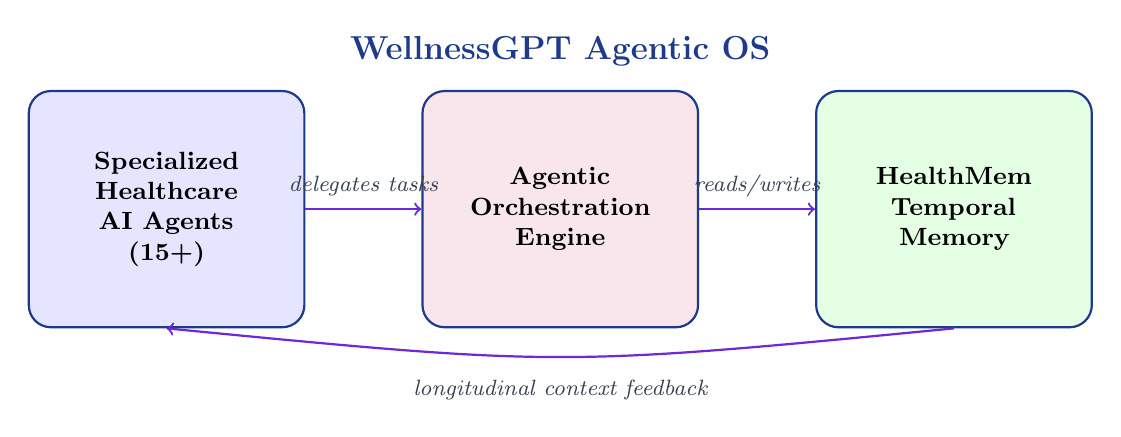
\begin{tikzpicture}[
    pillar/.style={rectangle, rounded corners=8pt, draw=primaryblue, fill=lightgray, 
                   minimum width=3.5cm, minimum height=3cm, text centered, text width=3cm,
                   thick, font=\small\bfseries},
    arrow/.style={->, thick, color=accentpurple},
    label/.style={font=\footnotesize\itshape, color=darkgray}
]

\node[pillar, fill=blue!10] (agents) at (0,0) {Specialized\\Healthcare\\AI Agents\\(15+)};
\node[pillar, fill=purple!10] (engine) at (5,0) {Agentic\\Orchestration\\Engine};
\node[pillar, fill=green!10] (mem) at (10,0) {HealthMem\\Temporal\\Memory};

\draw[arrow] (agents) -- (engine);
\draw[arrow] (engine) -- (mem);
\draw[arrow] (mem.south) .. controls (5,-2) .. (agents.south);

\node[label] at (2.5, 0.3) {delegates tasks};
\node[label] at (7.5, 0.3) {reads/writes};
\node[label] at (5, -2.3) {longitudinal context feedback};

\node[font=\large\bfseries\color{primaryblue}] at (5, 2) {WellnessGPT Agentic OS};

\end{tikzpicture}
\caption{High-level Architecture: Three-Pillar Model}
\end{figure}

%-----------------------------------------------------------
\subsection{Pillar 1: Specialized Healthcare AI Agents}

\subsubsection{Overview}

WellnessGPT provides a library of \textbf{15+ pre-trained, domain-specialized AI agents}. Each agent is fine-tuned for a specific clinical or administrative task, rather than being a general-purpose model. This specialization dramatically improves accuracy and reliability within its domain.

\subsubsection{Agent Catalogue}

\begin{table}[H]
\centering
\renewcommand{\arraystretch}{1.3}
\begin{tabularx}{\textwidth}{lX}
\toprule
\textbf{Agent Name} & \textbf{Function} \\
\midrule
Triage Agent          & Assesses patient-reported symptoms, determines urgency level, routes to correct department \\
Appointment Scheduling Agent & Books, reschedules, and cancels appointments; sends reminders \\
Care Planning Agent   & Generates personalized care plans based on diagnosis, history, and guidelines \\
Clinical Documentation Agent & Auto-generates clinical notes, SOAP notes, discharge summaries \\
Follow-up Agent       & Proactively contacts patients post-visit for status checks \\
Adherence Agent       & Monitors medication and treatment compliance; sends nudges \\
Discharge Agent       & Manages hospital discharge process and post-care handoffs \\
Health Claims Agent   & Processes, validates, and adjudicates health insurance claims \\
Billing / RCM Agent   & Revenue cycle management, billing automation, denial management \\
Patient Triage Agent  & Pre-visit symptom collection and urgency classification \\
Diagnostic Support Agent & Assists clinicians with differential diagnosis suggestions \\
Prescription Agent    & Processes and validates prescription requests \\
Health Campaign Agent & Executes targeted preventive health outreach campaigns \\
Consultation Agent    & Facilitates AI-assisted and human doctor consultations \\
Pharmacy Agent        & Digital pharmacy integrations and medicine delivery coordination \\
\bottomrule
\end{tabularx}
\caption{WellnessGPT Healthcare AI Agent Catalogue}
\end{table}

\subsubsection{Agent Design Principles}

\begin{itemize}[noitemsep]
    \item \textbf{Domain-Specific Fine-Tuning:} Each agent is trained on medical datasets relevant to its specialty, not on general web data alone
    \item \textbf{Plug-and-Play Integration:} Agents connect to hospital EHR/HMIS systems without requiring custom development
    \item \textbf{Multilingual Support:} Agents communicate in regional Indian languages as well as English
    \item \textbf{Empathy-Driven Design:} Conversational tone is calibrated for patient comfort and trust
    \item \textbf{Department Customization:} Each agent can be further fine-tuned to a specific hospital's data, departments, and patient demographics
    \item \textbf{Digital Workforce:} Collectively, the agents function as a ``digital workforce'' capable of operating 24/7 across all departments
\end{itemize}

%-----------------------------------------------------------
\subsection{Pillar 2: Agentic Orchestration Engine}

\subsubsection{Overview}

The Orchestration Engine is the \textbf{central nervous system} of WellnessGPT. It coordinates all agents, manages workflow routing, enforces policies, and maintains the integrity of multi-step clinical processes. Without this layer, individual agents would operate in silos without awareness of broader patient context or departmental state.

\subsubsection{Core Capabilities}

\begin{enumerate}
    \item \textbf{Multi-Agent Orchestration:}
    The engine coordinates real-time collaboration between multiple agents. For example, the Triage Agent's output automatically triggers the Care Planning Agent, which feeds into the Billing Agent — all without manual handoffs.

    \item \textbf{Policy and Consent Enforcement:}
    Built-in compliance logic ensures agents follow clinical protocols, patient consent boundaries, and institutional policies at every step.

    \item \textbf{Context Sharing Across Agents:}
    Agents share rich context (patient history, current flags, prior decisions) within a session and across sessions via HealthMem.

    \item \textbf{Human-in-the-Loop (HITL) Oversight:}
    Configurable checkpoints allow clinicians to review, approve, or override AI decisions before they are acted upon — critical for high-stakes decisions.

    \item \textbf{Audit-Ready Event Tracking:}
    Every agent action, decision point, and data access is logged with timestamps and metadata for full regulatory auditability.

    \item \textbf{Governance Dashboard:}
    A centralized monitoring interface shows the status of all active agents, recent decisions, flagged cases, and compliance metrics.

    \item \textbf{EHR / HMIS Integration Layer:}
    The engine provides standardized API connectors to systems like EPIC, OpenMRS, and custom HMIS implementations.
\end{enumerate}

\subsubsection{Orchestration Flow Diagram}

\begin{figure}[H]
\centering
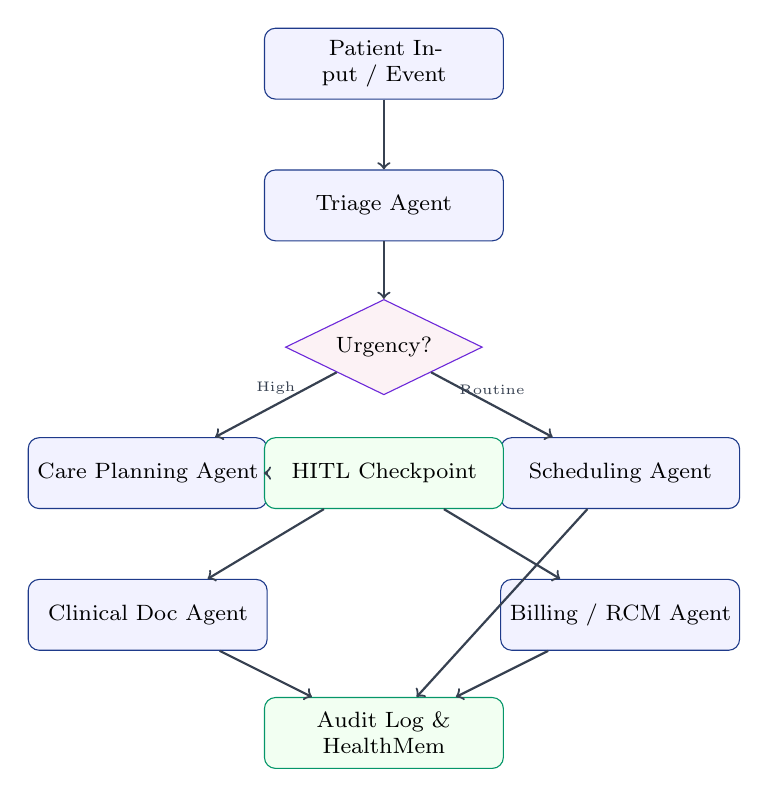
\begin{tikzpicture}[
    box/.style={rectangle, rounded corners=4pt, draw=primaryblue, fill=blue!5, 
                minimum width=2.8cm, minimum height=0.9cm, text centered, 
                text width=2.8cm, font=\footnotesize},
    decision/.style={diamond, draw=accentpurple, fill=purple!5, 
                     minimum width=2.5cm, minimum height=0.9cm, 
                     text centered, font=\footnotesize, aspect=2},
    arr/.style={->, thick, color=darkgray},
    hlbox/.style={rectangle, rounded corners=4pt, draw=successgreen, fill=green!5,
                  minimum width=2.8cm, minimum height=0.9cm, text centered,
                  text width=2.8cm, font=\footnotesize}
]

\node[box] (patient) at (0,0) {Patient Input / Event};
\node[box] (triage) at (0,-1.8) {Triage Agent};
\node[decision] (decision) at (0,-3.6) {Urgency?};
\node[box] (care) at (-3,-5.2) {Care Planning Agent};
\node[box] (routine) at (3,-5.2) {Scheduling Agent};
\node[box] (doc) at (-3,-7) {Clinical Doc Agent};
\node[box] (billing) at (3,-7) {Billing / RCM Agent};
\node[hlbox] (hitl) at (0,-5.2) {HITL Checkpoint};
\node[hlbox] (audit) at (0,-8.5) {Audit Log \& HealthMem};

\draw[arr] (patient) -- (triage);
\draw[arr] (triage) -- (decision);
\draw[arr] (decision) -- node[above, font=\tiny]{High} (care);
\draw[arr] (decision) -- node[above, font=\tiny]{Routine} (routine);
\draw[arr] (care) -- (hitl);
\draw[arr] (hitl) -- (doc);
\draw[arr] (hitl) -- (billing);
\draw[arr] (doc) -- (audit);
\draw[arr] (billing) -- (audit);
\draw[arr] (routine) -- (audit);

\end{tikzpicture}
\caption{Multi-Agent Orchestrated Workflow Example}
\end{figure}

%-----------------------------------------------------------
\subsection{Pillar 3: HealthMem --- Agentic Temporal Memory}

\subsubsection{Overview}

HealthMem is WellnessGPT's most technically distinct component. It is a \textbf{hybrid, multi-layered memory architecture} designed specifically for clinical data. Unlike a simple database or a RAG (Retrieval-Augmented Generation) vector store, HealthMem fuses three distinct memory types to enable comprehensive, context-aware patient understanding.

\subsubsection{Memory Architecture}

\begin{table}[H]
\centering
\renewcommand{\arraystretch}{1.4}
\begin{tabularx}{\textwidth}{llX}
\toprule
\textbf{Memory Layer} & \textbf{Technology Type} & \textbf{Purpose \& Capability} \\
\midrule
\textbf{Vector Store} & Semantic embedding search & 
  Fuzzy, semantic recall. Answers questions like: ``What complaints has this patient had over the last 6 months?'' Enables similarity-based retrieval across unstructured clinical notes. \\
\midrule
\textbf{Knowledge Graph} & Entity-relationship graph database & 
  Structured reasoning. Captures relationships between entities: diagnoses $\leftrightarrow$ medications $\leftrightarrow$ allergies $\leftrightarrow$ procedures. Enables reasoning like: ``This medication conflicts with the patient's known allergy.'' \\
\midrule
\textbf{KV Cache} & Key-value in-memory store & 
  Ultra-fast recall of frequently accessed, structured data (latest vitals, recent visit notes). Achieves \textbf{sub-150ms latency} for real-time clinical interactions. \\
\bottomrule
\end{tabularx}
\caption{HealthMem: Three-Layer Memory Architecture}
\end{table}

\subsubsection{Key Technical Properties}

\begin{itemize}[noitemsep]
    \item \textbf{Sub-150ms Recall Latency:} Fast enough for real-time conversational AI in clinical settings
    \item \textbf{Longitudinal Patient Timelines:} Stores and reasons across a patient's complete medical history, not just the current session
    \item \textbf{Timeline \& Importance-Based Prioritization:} More clinically relevant memories are surfaced first using intelligent ranking
    \item \textbf{FHIR-Aligned Data Model:} All stored data conforms to HL7 FHIR standards for interoperability
    \item \textbf{EPIC-Compatible:} Integrates natively with EPIC EHR systems
    \item \textbf{Full Encryption:} Data encrypted at rest and in transit
    \item \textbf{HIPAA \& ABDM Compliant:} Meets both US and Indian national health data regulations
    \item \textbf{Cross-Agent Memory:} Memory is shared across all agents operating on the same patient, enabling coherent multi-agent behavior
\end{itemize}

\newpage

%-----------------------------------------------------------
% Section 4: System Flow
%-----------------------------------------------------------
\section{System Flow and User Journey}

\subsection{Enterprise (B2B) Deployment Flow}

The primary market for WellnessGPT is enterprise healthcare organizations. The deployment journey follows these phases:

\begin{enumerate}
    \item \textbf{Discovery:} A healthcare organization (hospital chain, insurer, digital health company) visits \texttt{wellness-gpt.com}, learns about the platform's capabilities, and clicks the \emph{``Talk with our team''} call-to-action.

    \item \textbf{Inquiry \& Needs Assessment:} The prospect completes a Google Form inquiry. HeyDoc AI's team conducts a discovery call to understand the organization's existing systems, workflows, pain points, and compliance requirements.

    \item \textbf{Agent Configuration:} Using the \textbf{Care Agent Studio} — WellnessGPT's enterprise dashboard — the organization selects which agents to deploy, configures their parameters, and initiates fine-tuning on institutional data (patient records, departmental workflows, clinical protocols).

    \item \textbf{System Integration:} The Orchestration Engine's API connectors are used to integrate with the organization's existing EHR/HMIS/billing systems. HealthMem begins ingesting and indexing historical patient data into the three-layer memory architecture.

    \item \textbf{Go-Live \& Orchestration:} Agents go live and begin handling tasks semi-autonomously. The Orchestration Engine routes work between agents following configured clinical workflows. Human-in-the-loop checkpoints are activated at configured decision points.

    \item \textbf{Monitoring \& Governance:} The Governance Dashboard provides real-time visibility into all agent activities, decision logs, compliance metrics, and system health. Full audit trails are maintained for regulatory review.
\end{enumerate}

\subsection{Patient (B2C) Flow via HeyDoc App}

\begin{enumerate}[noitemsep]
    \item Patient downloads the \textbf{HeyDoc App} (iOS or Android)
    \item Patient creates or links an \textbf{ABHA ID} (Ayushman Bharat Health Account — India's national digital health ID)
    \item Patient uploads medical records, lab reports, and prescriptions
    \item WellnessGPT-powered features analyze the uploads and generate:
    \begin{itemize}[noitemsep]
        \item Plain-language health summaries
        \item Medication reminders and adherence tracking
        \item Doctor and specialist recommendations
        \item Service recommendations (digital pharmacy, consultations)
    \end{itemize}
    \item HealthMem builds and maintains a longitudinal memory profile for the patient
    \item Each subsequent interaction is personalized based on the growing memory graph
\end{enumerate}

\subsection{Integration Flow Summary}

\begin{figure}[H]
\centering
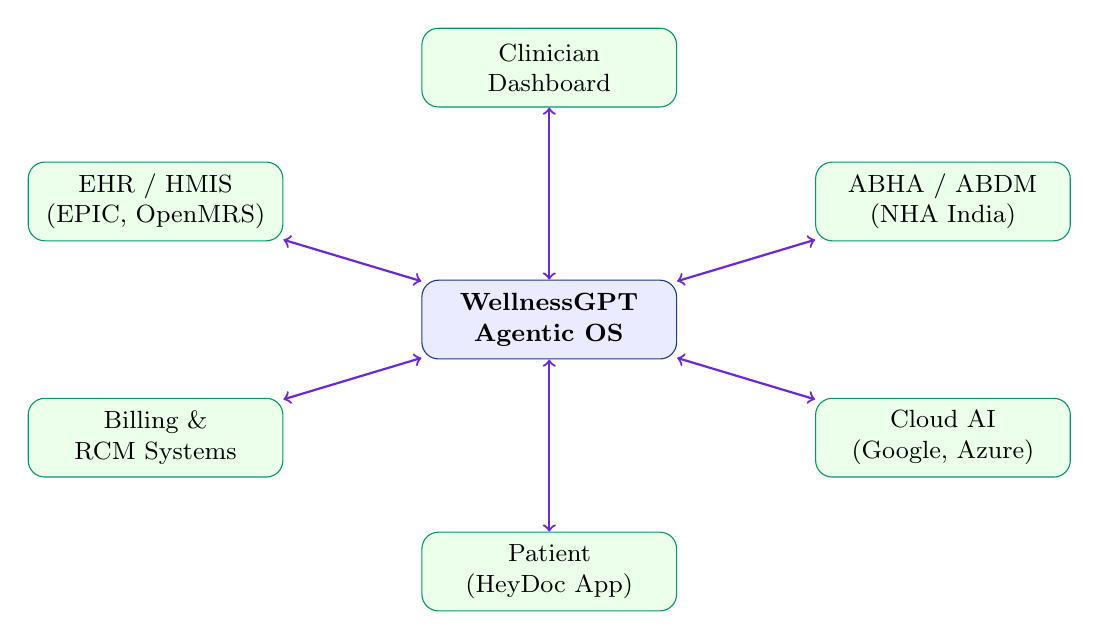
\begin{tikzpicture}[
    sys/.style={rectangle, rounded corners=6pt, draw=primaryblue, fill=blue!8, 
                minimum width=3.2cm, minimum height=1cm, text centered, 
                text width=3cm, font=\small\bfseries},
    ext/.style={rectangle, rounded corners=6pt, draw=successgreen, fill=green!8,
                minimum width=3.2cm, minimum height=1cm, text centered,
                text width=3cm, font=\small},
    arr/.style={<->, thick, color=accentpurple}
]

\node[sys] (os)       at (0,0)    {WellnessGPT\\Agentic OS};
\node[ext] (ehr)      at (-5, 1.5) {EHR / HMIS\\(EPIC, OpenMRS)};
\node[ext] (billing)  at (-5,-1.5) {Billing \&\\RCM Systems};
\node[ext] (abha)     at (5, 1.5)  {ABHA / ABDM\\(NHA India)};
\node[ext] (cloud)    at (5,-1.5)  {Cloud AI\\(Google, Azure)};
\node[ext] (patient)  at (0,-3.2)  {Patient\\(HeyDoc App)};
\node[ext] (clinician)at (0,3.2)   {Clinician\\Dashboard};

\draw[arr] (os) -- (ehr);
\draw[arr] (os) -- (billing);
\draw[arr] (os) -- (abha);
\draw[arr] (os) -- (cloud);
\draw[arr] (os) -- (patient);
\draw[arr] (os) -- (clinician);

\end{tikzpicture}
\caption{WellnessGPT Integration Ecosystem}
\end{figure}

\newpage

%-----------------------------------------------------------
% Section 5: Technology Stack
%-----------------------------------------------------------
\section{Underlying Technology Stack}

\subsection{Cloud \& AI Infrastructure}

\begin{table}[H]
\centering
\renewcommand{\arraystretch}{1.4}
\begin{tabularx}{\textwidth}{llX}
\toprule
\textbf{Provider} & \textbf{Program / Product} & \textbf{Role in WellnessGPT} \\
\midrule
Google Cloud    & Vertex AI, Google for Startups & Foundation model hosting, fine-tuning, ML infrastructure \\
Microsoft Azure & Azure AI, OpenAI on Azure, MS for Startups & LLM backend for clinical reasoning and NLP tasks \\
NVIDIA          & NVIDIA Inception Program, GPU compute & High-throughput inference acceleration for real-time agents \\
\bottomrule
\end{tabularx}
\caption{Cloud and AI Infrastructure Partners}
\end{table}

\subsection{Memory Stack (HealthMem)}

\begin{table}[H]
\centering
\renewcommand{\arraystretch}{1.4}
\begin{tabularx}{\textwidth}{lX}
\toprule
\textbf{Layer} & \textbf{Likely Technologies} \\
\midrule
Vector Store     & Weaviate / pgvector / Pinecone for semantic embedding storage and similarity search \\
Knowledge Graph  & Neo4j / Amazon Neptune / custom FHIR graph for entity-relationship clinical knowledge \\
KV Cache         & Redis / Memcached for in-memory key-value fast recall (\textless{}150ms latency) \\
Embedding Models & Domain-specific biomedical embedding models (e.g., BioBERT, MedBERT, or fine-tuned variants) \\
\bottomrule
\end{tabularx}
\caption{HealthMem Technology Stack}
\end{table}

\subsection{Healthcare Compliance Standards}

\begin{table}[H]
\centering
\renewcommand{\arraystretch}{1.4}
\begin{tabularx}{\textwidth}{llX}
\toprule
\textbf{Standard} & \textbf{Full Form} & \textbf{Significance} \\
\midrule
\textbf{FHIR} & Fast Healthcare Interoperability Resources & Global HL7 standard for structuring and exchanging healthcare data; ensures interoperability between systems \\
\textbf{HIPAA} & Health Insurance Portability and Accountability Act & US federal law governing protected health information (PHI) security and privacy \\
\textbf{ABDM} & Ayushman Bharat Digital Mission & India's national digital health ecosystem framework for health data exchange \\
\textbf{ABHA} & Ayushman Bharat Health Account & Unique patient health ID system under ABDM (like Aadhaar for health) \\
\textbf{NDHM} & National Digital Health Mission & Overarching policy framework for India's digital health infrastructure \\
\textbf{EPIC} & Electronic Practice Information Connector & Major US EHR system; WellnessGPT maintains EPIC compatibility \\
\bottomrule
\end{tabularx}
\caption{Healthcare Compliance and Interoperability Standards}
\end{table}

\subsection{Application Layer}

\begin{itemize}[noitemsep]
    \item \textbf{Care Agent Studio:} Enterprise web application for agent configuration, deployment, and monitoring (likely built on React/Next.js with a REST or GraphQL API backend)
    \item \textbf{Governance Dashboard:} Real-time monitoring interface for audit trails, agent status, and compliance metrics
    \item \textbf{HeyDoc Mobile App:} Consumer-facing iOS and Android application powered by WellnessGPT's agent infrastructure
    \item \textbf{API Layer:} RESTful APIs and webhooks for EHR/HMIS integration and third-party service connectivity
\end{itemize}

\newpage

%-----------------------------------------------------------
% Section 6: Services and Integrations
%-----------------------------------------------------------
\section{Services and Integrations}

\subsection{Integrated Service Ecosystem}

WellnessGPT connects with and enables the following service categories:

\begin{itemize}
    \item \textbf{Health Consultations:} AI-assisted and human doctor consultations mediated through the platform
    \item \textbf{Digital Pharmacy:} Prescription fulfillment and medicine delivery integrations
    \item \textbf{Product Recommendations:} Health supplements, devices, and wellness products
    \item \textbf{Health Campaigns:} Targeted preventive health outreach programs for patient populations
    \item \textbf{EHR Systems:} Read/write integration with EPIC, OpenMRS, and custom HMIS platforms
    \item \textbf{Billing Systems:} Insurance and revenue cycle management systems
    \item \textbf{National Health Authority (NHA):} Government-level integration with India's ABDM infrastructure
\end{itemize}

\subsection{Target Use Cases by Segment}

\begin{table}[H]
\centering
\renewcommand{\arraystretch}{1.4}
\begin{tabularx}{\textwidth}{lX}
\toprule
\textbf{Customer Segment} & \textbf{Key Use Cases} \\
\midrule
Multi-speciality Hospital Chains & End-to-end patient journey automation from triage through discharge and billing; clinical documentation; patient follow-up \\
Digital Health Companies         & Embedding AI-powered features (health records analysis, care plans, personalized health insights) into their consumer apps \\
Health Insurance \& Claim Processors & Automated claims intake, validation, adjudication, and denial management \\
Government / Public Health       & ABDM-integrated national health programs, preventive care campaigns, population health management \\
\bottomrule
\end{tabularx}
\caption{Target Customer Segments and Use Cases}
\end{table}

\newpage

%-----------------------------------------------------------
% Section 7: Competitive Differentiation
%-----------------------------------------------------------
\section{Competitive Differentiation}

\subsection{WellnessGPT vs. Generic LLM Deployments}

\begin{table}[H]
\centering
\renewcommand{\arraystretch}{1.5}
\begin{tabularx}{\textwidth}{lXX}
\toprule
\textbf{Dimension} & \textbf{Generic LLM (e.g., GPT-4)} & \textbf{WellnessGPT} \\
\midrule
Patient Memory        & None (stateless)              & Full longitudinal memory via HealthMem \\
Domain Specialization & General purpose               & 15+ clinical domain-specialized agents \\
Multi-Agent Support   & Single model                  & Coordinated multi-agent orchestration \\
Compliance            & Not built-in                  & HIPAA, ABDM, FHIR by design \\
EHR Integration       & Not available natively        & Native EHR/HMIS integration \\
Audit Trail           & Not possible                  & Full audit-ready governance dashboard \\
Human Oversight       & No structured HITL            & Configurable human-in-the-loop checkpoints \\
Clinical Workflow     & No structure                  & Full workflow orchestration engine \\
Fine-tuning           & Generic or prompt-only        & Per-department, per-patient customization \\
Language Support      & English-primary               & Multilingual including Indian regional languages \\
\bottomrule
\end{tabularx}
\caption{Comparative Analysis: WellnessGPT vs. Generic LLMs}
\end{table}

\newpage

%-----------------------------------------------------------
% Section 8: Company and Ecosystem
%-----------------------------------------------------------
\section{Company Overview and Ecosystem}

\subsection{HeyDoc AI}

WellnessGPT is developed and operated by \textbf{HeyDoc AI} (legally: HeyDoc Healthtech Private Limited), an Indian healthtech startup. The company operates two distinct product lines:

\begin{itemize}
    \item \textbf{WellnessGPT} (\texttt{wellness-gpt.com}): Enterprise Agentic AI OS for healthcare organizations
    \item \textbf{HeyDoc App} (\texttt{heydoc.co.in}): Consumer-facing health management app for patients
\end{itemize}

\subsection{Team}

The HeyDoc AI team is composed of clinicians and technologists from premier Indian institutions:
\begin{itemize}[noitemsep]
    \item \textbf{IIT} (Indian Institute of Technology) — technology and engineering expertise
    \item \textbf{AIIMS} (All India Institute of Medical Sciences) — clinical domain expertise
\end{itemize}

\subsection{Backing and Partnerships}

\begin{table}[H]
\centering
\renewcommand{\arraystretch}{1.4}
\begin{tabularx}{\textwidth}{lX}
\toprule
\textbf{Partner / Backer} & \textbf{Nature of Support} \\
\midrule
Google for Startups      & Cloud infrastructure, Vertex AI access, startup support program \\
Microsoft for Startups   & Azure AI credits, enterprise tooling, OpenAI on Azure access \\
NVIDIA Inception Program & GPU compute resources, AI accelerator program membership \\
National Health Authority (NHA) & Government of India healthcare ecosystem collaboration \\
\bottomrule
\end{tabularx}
\caption{Strategic Backers and Partners}
\end{table}

\subsection{Contact Information}

\begin{itemize}[noitemsep]
    \item \textbf{Business Email:} \href{mailto:business@heydoc.co.in}{business@heydoc.co.in}
    \item \textbf{Phone:} +91 9027391190
    \item \textbf{Website:} \href{https://wellness-gpt.com}{wellness-gpt.com}
    \item \textbf{Consumer App:} \href{https://heydoc.co.in}{heydoc.co.in}
    \item \textbf{Social:} Twitter/X, LinkedIn, Instagram, Facebook, YouTube
\end{itemize}

\newpage

%-----------------------------------------------------------
% Section 9: FAQ Summary
%-----------------------------------------------------------
\section{Frequently Asked Questions (Platform FAQ)}

The following FAQs are sourced directly from the WellnessGPT website:

\begin{enumerate}
    \item \textbf{What is WellnessGPT?}\\
    WellnessGPT is an Agentic AI Operating System for healthcare with specialized agents, orchestration, and longitudinal memory.

    \item \textbf{What kinds of organizations does it serve?}\\
    It powers semi-autonomous workflows across hospital chains, digital health companies, insurers, and claims processors with governed automation.

    \item \textbf{How do the components work together?}\\
    The Agentic Orchestration Engine coordinates multi-agent workflows, while HealthMem provides structured, longitudinal patient memory for context-aware decisions.

    \item \textbf{Is it compliant with healthcare regulations?}\\
    WellnessGPT is built for regulated ecosystems with ABHA and FHIR alignment, secure memory architecture, and audit-ready workflows.
\end{enumerate}

\newpage

%-----------------------------------------------------------
% Section 10: Conclusion
%-----------------------------------------------------------
\section{Conclusion}

WellnessGPT represents a \textbf{paradigm shift in healthcare AI} — moving from simple chatbot-style LLM interactions to a fully orchestrated, memory-enabled, compliance-first \emph{Agentic AI Operating System}. Its three-pillar architecture of Specialized Agents, Orchestration Engine, and HealthMem Temporal Memory addresses the fundamental gaps that make generic LLMs unsuitable for clinical deployment.

By combining:
\begin{itemize}[noitemsep]
    \item \textbf{Domain specificity} (15+ fine-tuned clinical agents)
    \item \textbf{Coordinated intelligence} (multi-agent orchestration)
    \item \textbf{Persistent memory} (longitudinal patient context via HealthMem)
    \item \textbf{Regulatory compliance} (HIPAA, FHIR, ABDM by design)
\end{itemize}

WellnessGPT positions itself as the \textbf{infrastructure layer for the next generation of digital healthcare} — not just an AI tool on top of existing systems, but the intelligent OS that drives the entire healthcare operation. With strong industry backing from Google, Microsoft, and NVIDIA, and a close partnership with India's National Health Authority, WellnessGPT is well-positioned to become the standard Agentic AI infrastructure for healthcare organizations in India and beyond.

\vspace{1cm}

\begin{mdframed}[backgroundcolor=lightgray, linecolor=primaryblue, linewidth=1pt, roundcorner=5pt]
\textbf{Key Takeaways:}
\begin{itemize}[noitemsep]
    \item WellnessGPT is an Agentic AI OS, not a chatbot
    \item Three pillars: Specialized Agents + Orchestration Engine + HealthMem
    \item HealthMem achieves sub-150ms recall with hybrid Vector + Graph + KV architecture
    \item Fully compliant: HIPAA, FHIR, ABDM, ABHA
    \item Backed by Google, Microsoft, and NVIDIA
    \item Target market: hospital chains, insurers, digital health companies
    \item Business model: Enterprise custom pricing; consumer app via HeyDoc
\end{itemize}
\end{mdframed}

\vspace{1cm}

\hrule
\vspace{0.3cm}
\small
\textbf{Source:} WellnessGPT website (\href{https://wellness-gpt.com}{wellness-gpt.com}) and HeyDoc consumer platform (\href{https://heydoc.co.in}{heydoc.co.in}). Research conducted March 2026.\\
\textbf{Copyright:} \textcopyright~2026 HeyDoc AI --- All Rights Reserved. \textit{Agentic AI Infrastructure for Healthcare Systems.}

\end{document}
